\chapter{Virologia}\label{ch:b3:virology}

Há uns $10^{31}$ partículas de \omterm{def:b3:virology:virus}{vírus} na Terra, dez para cada célula, e
no mar elas matam um quinto de todas as bactérias por dia. Um \omterm{def:b3:virology:virus}{vírus} não
é uma célula: não tem metabolismo, não tem ribossomos, não tem como
fazer nada sozinho. É um genoma --- tão curto quanto dois genes, tão
longo quanto dois mil --- envolto num casco de proteína, que entra numa
célula e volta a maquinaria dela para fazer cópias de si mesmo. A gripe
de 1918 matou cinquenta milhões de pessoas; a varíola, que matou
trezentos milhões só no século XX, foi erradicada em 1980 por uma
\omterm{def:b3:virology:drugs}{vacina} experimentada pela primeira vez em 1796; e um coronavírus que
passou aos humanos em 2019 teve seu genoma sequenciado em semanas, uma
\omterm{def:b3:virology:drugs}{vacina} desenhada poucos dias depois disso e fármacos contra sua
protease em dois anos. Este capítulo trata do que são os \omterm{def:b3:virology:virus}{vírus} e de
como são classificados pela química de seus genomas, de como se
multiplicam, da cinética de uma infecção dentro de um hospedeiro --- que
um par de equações diferenciais descreve bem o bastante para ter mudado
o tratamento da aids ---, de sua evolução e de como são combatidos.

\section{O que é um vírus}

\begin{definition}[Vírus]\label{def:b3:virology:virus}
\index{vírus}\index{capsídeo}\index{envelope}\index{vírion}\index{classificação de Baltimore}
Um \emph{vírus} é um parasito intracelular obrigatório constituído de
um genoma de ácido nucleico --- DNA ou RNA, de fita simples ou dupla,
linear ou circular, uma molécula ou várias --- empacotado num
\emph{capsídeo} proteico e, em muitos casos, envolto num
\emph{envelope} tomado de uma membrana do hospedeiro e cravejado de
glicoproteínas virais. A partícula infecciosa completa é o
\emph{vírion}, de \qtyrange{20}{300}{nm} na maioria (uns poucos vírus
gigantes chegam a um micrômetro). Os capsídeos são construídos de
muitas cópias de uma ou de umas poucas proteínas dispostas com simetria
helicoidal (um bastão, como no vírus do mosaico do tabaco) ou
icosaédrica (um casco de $60T$ subunidades, $T = 1, 3, 4, 7,\dots$). A
\emph{classificação de Baltimore} agrupa os vírus pela rota do genoma
até o RNA mensageiro: I, DNA de fita dupla (herpes, varíola,
adenovírus, a maioria dos fagos); II, DNA de fita simples
(parvovírus); III, RNA de fita dupla (rotavírus); IV, RNA de fita
positiva, ele próprio um mensageiro (poliovírus, hepatite C, os
coronavírus); V, RNA de fita negativa, complementar ao mensageiro
(influenza, sarampo, raiva, Ebola); VI, RNA transcrito reversamente em
DNA (os retrovírus, o HIV); VII, DNA replicado por um intermediário de
RNA (hepatite B). Toda classe exceto a I precisa trazer ou codificar
uma enzima que a célula não tem --- uma RNA-polimerase dependente de
RNA, uma transcriptase reversa ---, e essas enzimas são os alvos da
maioria dos \omterm{def:b3:virology:drugs}{antivirais}.
\end{definition}

\begin{proof}[Evidência]
Ivanovsky (1892) e Beijerinck (1898) mostraram que a doença do mosaico
do tabaco era transmitida por seiva passada por filtros que retinham
todas as bactérias --- um \emph{contagium vivum fluidum}, um fluido
infeccioso vivo. Stanley (1935) cristalizou o agente, o \omterm{def:b3:virology:virus}{vírus} do
mosaico do tabaco, e mostrou que ele era proteína com (como Bawden e
Pirie descobriram) \qty{5}{\%} de RNA. Hershey e Chase (1952) marcaram
a proteína de um bacteriófago com $^{35}$S e seu DNA com $^{32}$P,
deixaram-no infectar \emph{E.~coli}, arrancaram os cascos vazios num
liquidificador e encontraram o $^{32}$P dentro das células e o
$^{35}$S fora: o DNA entra e a proteína fica para trás, de modo que é o
DNA que carrega as instruções. Fraenkel-Conrat (1955) desmontou o
\omterm{def:b3:virology:virus}{vírus} do mosaico do tabaco em proteína e RNA e remontou partículas
infecciosas com o RNA de uma linhagem e a proteína de outra; a prole era
da linhagem do RNA.
\end{proof}

\begin{proposition}[Economia genética: por que os capsídeos são simétricos]\label{prop:b3:virology:economy}
\index{economia genética}
Um \omterm{def:b3:virology:virus}{capsídeo} precisa encerrar o genoma que o codifica. Uma proteína de
massa $m$ precisa de cerca de $m/\qty{110}{Da}$ códons, isto é, de
$3m/110$ nucleotídeos, um trecho de RNA que pesa cerca de
$3m/110\times\qty{330}{Da} = 9m$: qualquer proteína é codificada por um
ácido nucleico nove vezes mais pesado que ela. Um casco feito de uma
\emph{única} molécula de proteína que encerrasse um genoma teria de
encerrar um genoma nove vezes mais pesado que ele apenas para
codificar-se, e um casco não consegue conter nove vezes sua própria
massa de ácido nucleico em densidade biológica. A saída, vista por
Crick e Watson (1956), é construir o casco com muitas cópias de uma
proteína pequena: o \omterm{def:b3:virology:virus}{vírus} do mosaico do tabaco codifica uma proteína de
casco de \qty{17.5}{kDa} em \qty{480}{nt} de seu genoma de
\qty{6400}{nt} e usa $2130$ cópias dela. Subunidades idênticas que se
empacotam de modo idêntico precisam estar dispostas simetricamente, e
por isso os \omterm{def:b3:virology:virus}{capsídeos} virais são hélices ou icosaedros; a mesma
economia lhes dá a capacidade de automontagem, já que cada subunidade
só precisa reconhecer suas vizinhas.
\end{proposition}
\begin{proof}
A razão de massas decorre de um códon ser três nucleotídeos de cerca de
\qty{330}{Da} cada e um resíduo cerca de \qty{110}{Da}:
$3\times 330/110 =
9$. Um \omterm{def:b3:virology:virus}{capsídeo} de uma única proteína de
\qty{40}{MDa} encerraria \qty{360}{MDa} de ácido nucleico, uma esfera
de raio de cerca de \qty{50}{nm} na densidade de ácido nucleico, ao
passo que a própria proteína faria um casco de cerca de \qty{2}{nm} de
espessura e do mesmo raio --- geometricamente possível, mas um único
polipeptídeo de $360\,000$ resíduos que se enovelasse corretamente não
é, e uma mutação o destruiria. Com $n$ subunidades idênticas, o custo
de codificação cai por $n$ e o volume encerrado não muda.
\end{proof}

\begin{omfigure}
\begin{tikzpicture}[every node/.style={font=\scriptsize}, >=stealth]
  \node[draw, thick, rounded corners, fill=omMeth!30, minimum width=2.4cm] (mrna) at (0,0) {mRNA $\to$ proteína};
  \node[draw, thick, rounded corners, fill=omDef!20, align=center] (I) at (-5.8,3.6) {I: DNAds\\herpes, varíola, fago T4};
  \node[draw, thick, rounded corners, fill=omDef!20, align=center] (II) at (-2.0,3.6) {II: DNAss\\parvovírus};
  \node[draw, thick, rounded corners, fill=omThm!20, align=center] (III) at (2.0,3.6) {III: RNAds\\rotavírus};
  \node[draw, thick, rounded corners, fill=omThm!20, align=center] (IV) at (5.8,3.6) {IV: RNA(+)\\poliovírus, hepatite C,\\coronavírus};
  \node[draw, thick, rounded corners, fill=omThm!20, align=center] (V) at (-5.6,-3.4) {V: RNA($-$)\\influenza, sarampo,\\raiva, Ebola};
  \node[draw, thick, rounded corners, fill=omProp!30, align=center] (VI) at (0,-3.4) {VI: RNA $\to$ DNA\\retrovírus (HIV)};
  \node[draw, thick, rounded corners, fill=omProp!30, align=center] (VII) at (5.6,-3.4) {VII: DNA via RNA\\hepatite B};
  \node[below, font=\tiny, align=center, gray!50!black] at (-5.8,2.9) {RNA-polimerase do hospedeiro};
  \node[below, font=\tiny, align=center, gray!50!black] at (-2.0,3.05) {a segunda fita é feita,\\depois a transcrição};
  \node[below, font=\tiny, align=center, gray!50!black] at (2.0,3.05) {RNA-polimerase viral\\dentro da partícula};
  \node[below, font=\tiny, align=center, gray!50!black] at (5.8,2.75) {o genoma é o mRNA};
  \node[above, font=\tiny, align=center, gray!50!black] at (-5.6,-2.55) {a polimerase viral o copia};
  \node[above, font=\tiny, align=center, gray!50!black] at (0,-2.85) {transcriptase reversa, integração,\\depois a polimerase do hospedeiro};
  \node[above, font=\tiny, align=center, gray!50!black] at (5.6,-2.85) {transcrição do DNA};
  \foreach \c in {I,II,III,IV,V,VI,VII} \draw[->, thick] (\c) -- (mrna);
\end{tikzpicture}

{\small As sete classes de Baltimore, ordenadas pela rota do genoma até
o RNA mensageiro. Toda classe, exceto a I, precisa de uma enzima que a
célula hospedeira não fornece --- o alvo natural de um \omterm{def:b3:virology:drugs}{antiviral}.}
\end{omfigure}

\begin{omfigure}
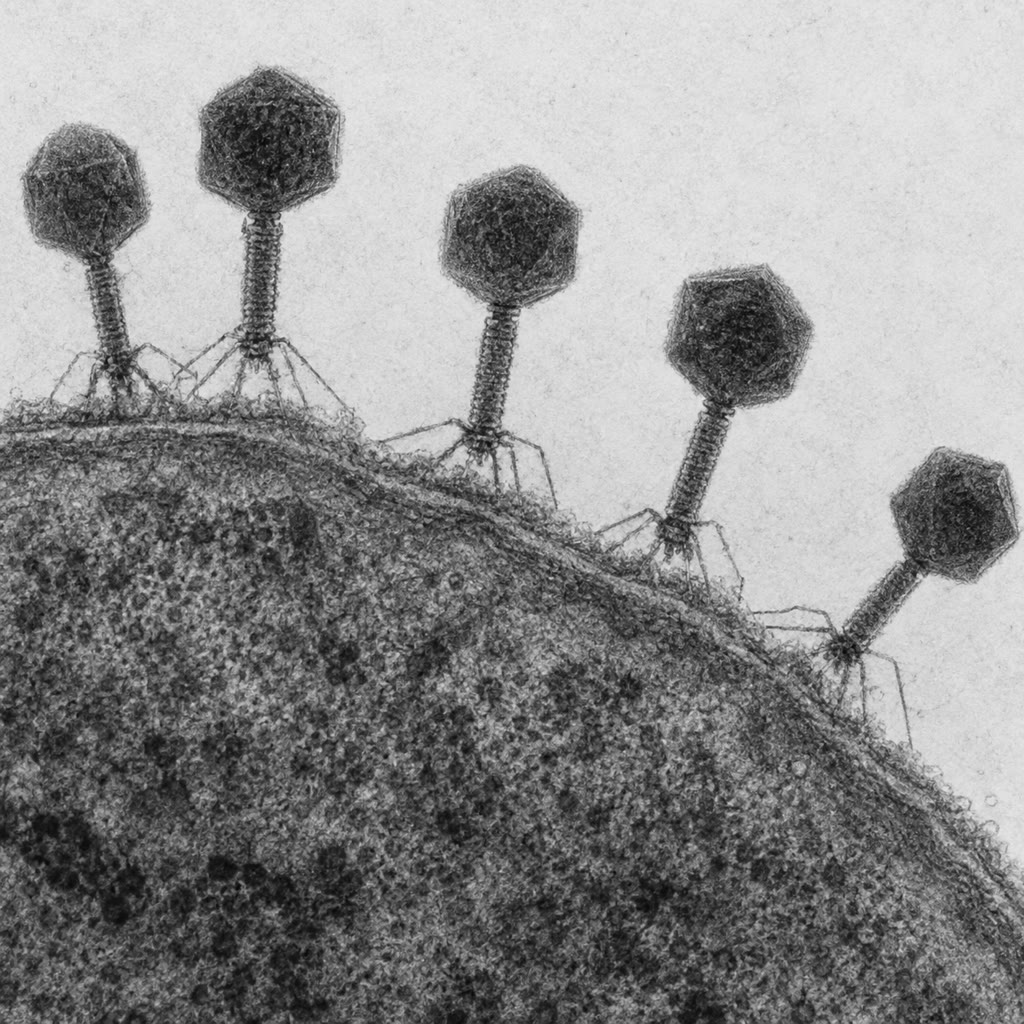
\includegraphics[width=0.36\linewidth]{images/book5/ai/b5-13-phage-tem.jpg}\hspace{0.04\linewidth}
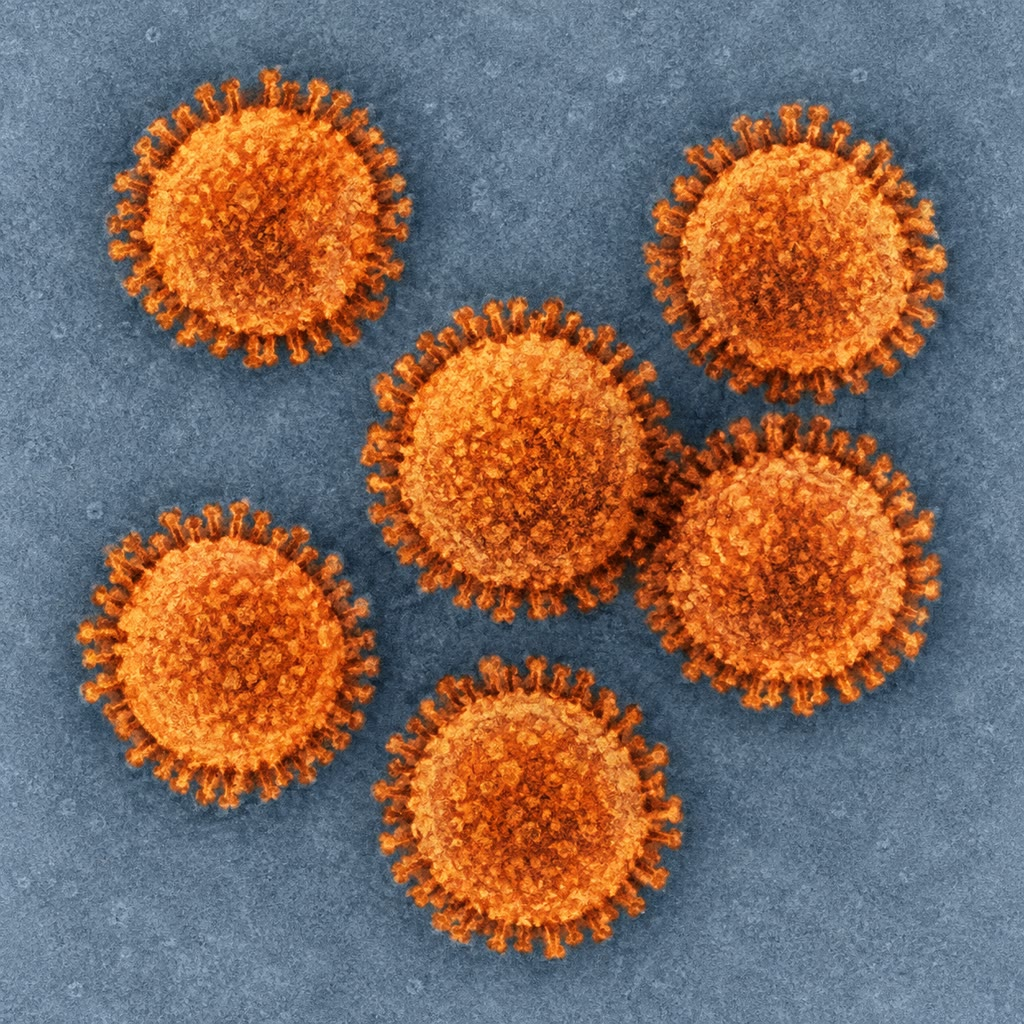
\includegraphics[width=0.36\linewidth]{images/book5/ai/b5-13-influenza-virions.jpg}

{\small À esquerda: bacteriófagos presos por suas fibras caudais a uma
bactéria, com cada cabeça sendo um \omterm{def:b3:virology:virus}{capsídeo} icosaédrico de DNA. À
direita: \omterm{def:b3:virology:virus}{vírions} de influenza, envelopados, com a superfície feita de
uma franja de espículas de hemaglutinina e neuraminidase.}
\end{omfigure}

\section{Como um vírus se multiplica}

\begin{definition}[O ciclo de replicação]\label{def:b3:virology:cycle}
\index{ciclo de replicação viral}\index{receptor!viral}\index{lisogenia}\index{latência}
Todo \omterm{def:b3:virology:virus}{vírus} passa pelas mesmas etapas. A \emph{adesão} a um receptor
específico do hospedeiro --- o CD4 e um receptor de quimiocina para o
HIV, a ACE2 para os coronavírus da SARS, o ácido siálico para a
influenza, um \omterm{def:b3:bacteriology:envelope}{lipopolissacarídeo} ou uma porina para um fago ---, que
decide quais espécies e quais células o \omterm{def:b3:virology:virus}{vírus} pode infectar (seu
\emph{tropismo}). A \emph{entrada}: a fusão do \omterm{def:b3:virology:virus}{envelope} com a membrana
plasmática, ou a endocitose seguida de fusão de dentro do \omterm{def:b3:membrane-traffic:endocytosis}{endossomo}
ácido, ou, para um fago, a injeção do genoma através da parede. O
\emph{desnudamento}, a \emph{expressão} dos genes virais pela rota
específica da classe, e a \emph{replicação} do genoma, muitas vezes
numa fábrica que o \omterm{def:b3:virology:virus}{vírus} constrói no citoplasma ou no núcleo. A
\emph{montagem} de novos \omterm{def:b3:virology:virus}{capsídeos} em torno de novos genomas,
impulsionada pela automontagem das subunidades simétricas, e a
\emph{liberação}: por lise da célula, ou por brotamento através de uma
membrana, que fornece o \omterm{def:b3:virology:virus}{envelope}. Alguns \omterm{def:b3:virology:virus}{vírus} podem, em vez disso,
inserir seu genoma no do hospedeiro e esperar: a \emph{lisogenia} do
fago $\lambda$, cujo repressor o mantém silencioso até que o hospedeiro
seja danificado; a \emph{latência} dos herpesvírus em neurônios por uma
vida inteira e a do HIV como provírus em linfócitos~T em repouso, de
onde nenhum fármaco que aja sobre a replicação o remove.
\end{definition}

\begin{omfigure}
\begin{tikzpicture}[every node/.style={font=\scriptsize}, >=stealth]
  % cell
  \draw[very thick, omDef, fill=omDef!6] (0,0) ellipse (5.6 and 3.2);
  \draw[thick, omDef!70, fill=omDef!20] (1.8,0) ellipse (1.6 and 1.1); \node at (1.8,0.75) {núcleo};
  % virion outside
  \draw[thick, omProp, fill=omProp!30] (-7.2,1.6) circle (0.35); \foreach \a in {0,45,...,315} \draw[omProp, thick] (-7.2,1.6) ++(\a:0.35) -- ++(\a:0.15);
  \node[above] at (-7.2,2.1) {vírion};
  \draw[->, thick] (-6.8,1.4) -- (-5.7,0.9); \node[below, align=center] at (-6.6,1.0) {1. adere ao\\receptor};
  % entry
  \draw[thick, omProp] (-5.4,0.7) arc[start angle=140, end angle=40, radius=0.5];
  \node[below, align=center] at (-3.9,-0.2) {2. funde-se ou é endocitado;\\3. desnuda-se};
  % genome path
  \draw[omThm, very thick] (-3.4,0.2) .. controls (-2.6,0.6) .. (-1.8,0.4);
  \draw[->, thick] (-1.6,0.4) -- (-0.4,0.4);
  \node[above, align=center] at (-1.0,0.55) {4. expressa genes,\\replica o genoma};
  \draw[omThm, very thick] (-1.0,-0.5) -- (0.4,-0.5); \draw[omThm, very thick] (-1.0,-0.75) -- (0.4,-0.75); \draw[omThm, very thick] (-1.0,-1.0) -- (0.4,-1.0);
  % assembly
  \foreach \p in {(1.2,-1.6),(1.9,-1.9),(2.6,-1.5)} { \draw[thick, omProp, fill=omProp!30] \p circle (0.25); }
  \node[below, align=center] at (1.9,-2.2) {5. monta capsídeos\\em torno dos genomas};
  % budding
  \draw[thick, omProp, fill=omProp!30] (4.9,-1.7) circle (0.32); \draw[->, thick] (5.3,-1.75) -- (6.4,-2.0);
  \draw[thick, omProp, fill=omProp!30] (7.0,-2.2) circle (0.35); \foreach \a in {0,45,...,315} \draw[omProp, thick] (7.0,-2.2) ++(\a:0.35) -- ++(\a:0.15);
  \node[below, align=center] at (6.4,-2.6) {6. brota pela membrana\\(envelope) ou lisa a célula};
  % latency
  \draw[->, thick, dashed, omMeth!70!black] (-0.2,0.2) -- (0.9,0.2); \node[below, omMeth!70!black, align=center, font=\tiny] at (2.0,-0.05) {retrovírus: integram-se\\como provírus; latência};
\end{tikzpicture}

{\small O ciclo de replicação de um \omterm{def:b3:virology:virus}{vírus} envelopado: adesão a um
receptor, entrada e desnudamento, expressão e replicação na maquinaria
do hospedeiro, montagem e liberação por brotamento --- ou, no caso de um
retrovírus, integração no genoma do hospedeiro e silêncio.}
\end{omfigure}

\begin{method}[Contar partículas infecciosas: o ensaio de placas]\label{met:b3:virology:plaque}
\index{ensaio de placas}\index{título}
Para medir um estoque de \omterm{def:b3:virology:virus}{vírus}: (1) dilua-o em passos de dez vezes; (2)
misture cada diluição a um excesso de células hospedeiras --- bactérias
em ágar mole para um fago, uma monocamada de células em cultura para um
\omterm{def:b3:virology:virus}{vírus} animal; (3) incube: cada partícula infecciosa infecta uma célula,
a prole infecta as vizinhas, e depois de um ou dois dias um buraco
claro, uma \emph{placa}, marca o ponto; (4) conte as placas numa placa
de Petri que tenha de \numrange{30}{300} e multiplique pela diluição: é
o \emph{título} em unidades formadoras de placa (UFP) por mililitro.
Como cada placa é um clone de uma partícula, colhê-la dá um isolado
puro. A razão entre partículas físicas (contadas por microscopia
eletrônica ou PCR) e unidades formadoras de placa costuma estar bem
acima de um --- de dez a mil para muitos \omterm{def:b3:virology:virus}{vírus} animais ---, já que a
maioria das partículas é defeituosa ou não consegue infectar.
\end{method}

\begin{omfigure}
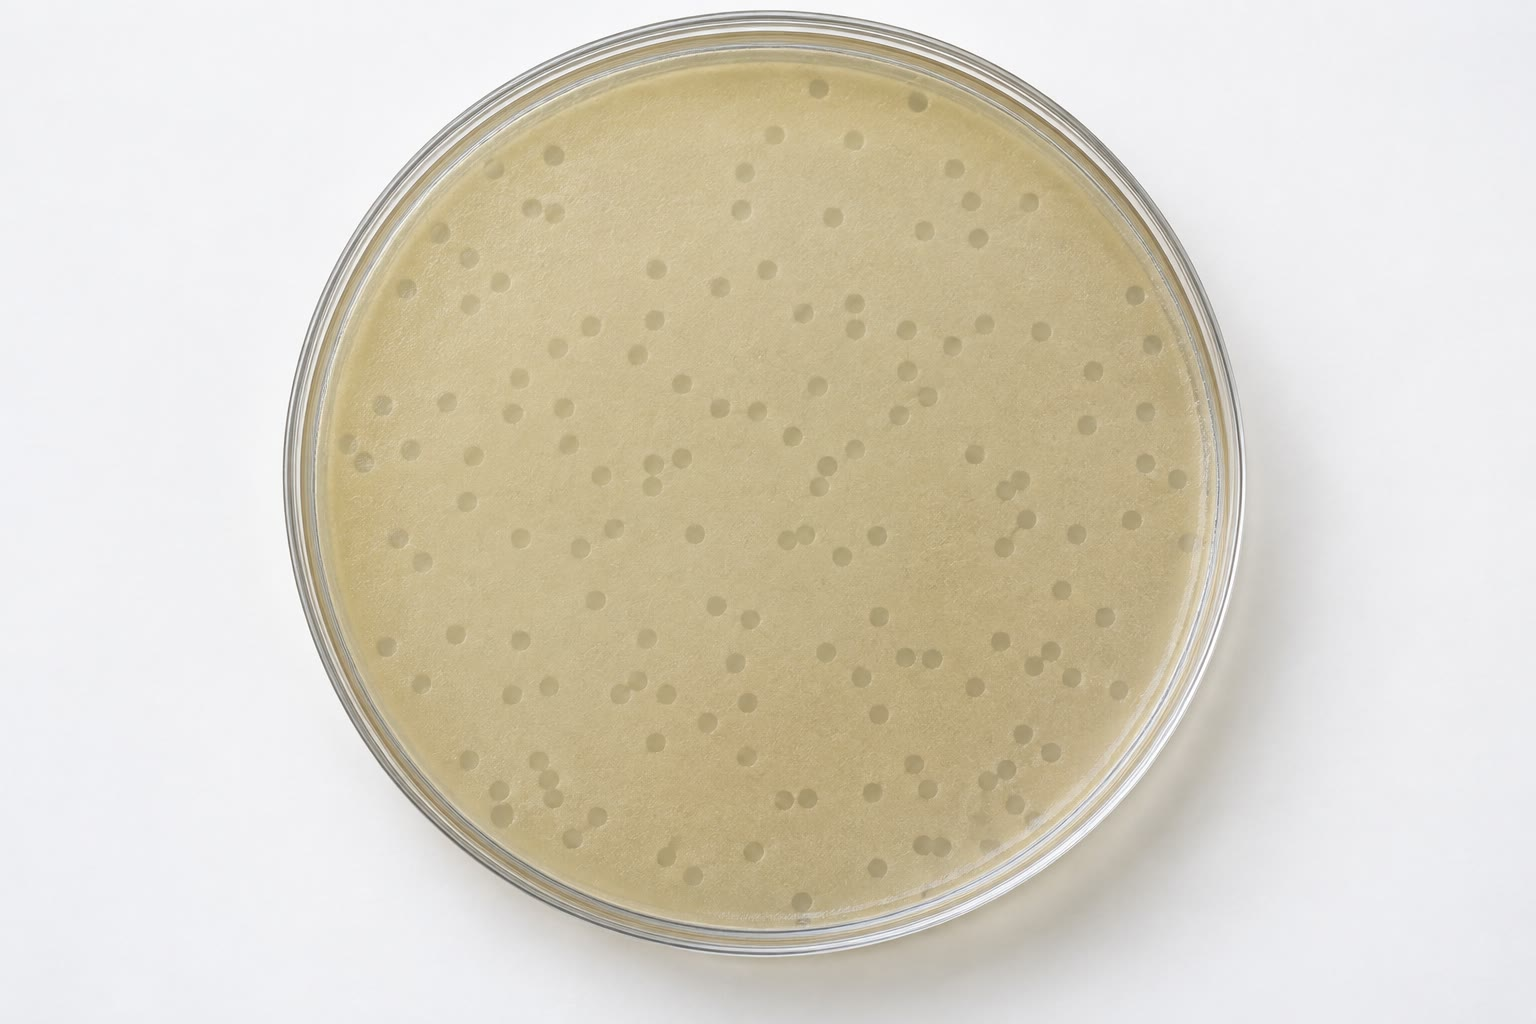
\includegraphics[width=0.46\linewidth]{images/book5/ai/b5-13-plaque-assay.jpg}\hspace{0.04\linewidth}
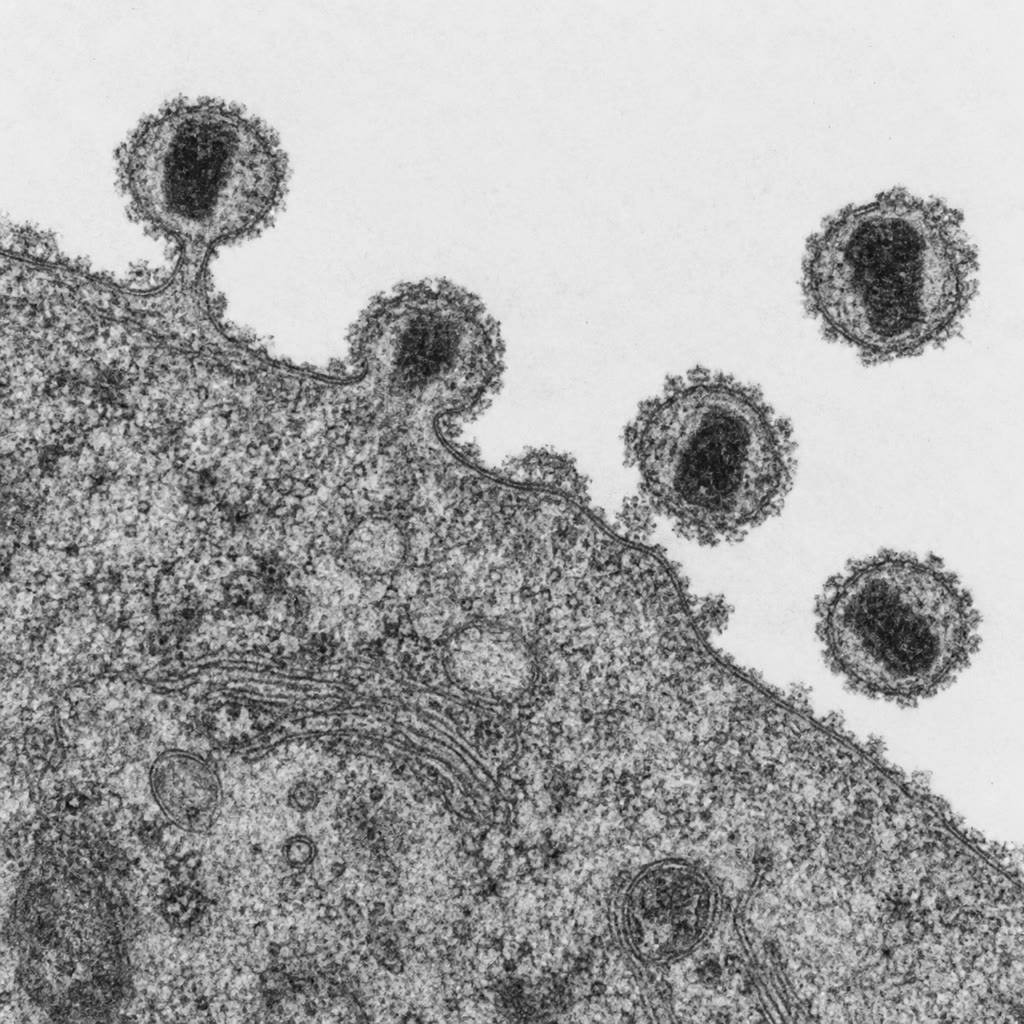
\includegraphics[width=0.36\linewidth]{images/book5/ai/b5-13-hiv-budding.jpg}

{\small À esquerda: placas num gramado bacteriano, cada uma uma zona
clara em que a prole de um fago lisou as células ao redor. À direita:
partículas de HIV brotando de um linfócito~T, tomando seu \omterm{def:b3:virology:virus}{envelope} da
membrana da célula.}
\end{omfigure}

\begin{theorem}[Dinâmica da infecção dentro de um hospedeiro]\label{thm:b3:virology:dynamics}
\index{número básico de reprodução!dentro do hospedeiro}\index{carga viral}\index{dinâmica viral}
Sejam $T$ a densidade de células-alvo suscetíveis, $I$ a de células
infectadas e $V$ a de \omterm{def:b3:virology:virus}{vírions} livres. Os \omterm{def:b3:virology:virus}{vírions} infectam alvos à taxa
$\beta TV$, as células infectadas produzem \omterm{def:b3:virology:virus}{vírions} à taxa $p$ cada uma
e morrem à taxa $\delta$, e os \omterm{def:b3:virology:virus}{vírions} livres são depurados à taxa $c$:
\[
\frac{\mathrm{d}I}{\mathrm{d}t} = \beta TV - \delta I, \qquad
\frac{\mathrm{d}V}{\mathrm{d}t} = pI - cV .
\]
Com $T$ mantido constante, a infecção cresce se o \emph{número básico de
reprodução} $R_{0} = \beta Tp/(c\delta)$ exceder $1$, e no estado
estacionário $V^{*} = p I^{*}/c$, com a produção equilibrando a
depuração. Se um fármaco interrompe todas as novas infecções em $t = 0$
($\beta \to 0$), os \omterm{def:b3:virology:virus}{vírions} decaem no início à taxa de depuração $c$ e
depois, uma vez que o \omterm{def:b3:virology:virus}{vírus} livre tenha caído ao nível que as células
infectadas restantes sustentam, à taxa de morte $\delta$ dessas
células:
\[
V(t) \approx V_{0}\,\frac{c\,e^{-\delta t} - \delta\,e^{-ct}}{c - \delta}
\;\longrightarrow\; V_{0}\,\frac{c}{c-\delta}\,e^{-\delta t}
\quad (t \gg 1/c).
\]
As duas inclinações da \omterm{thm:b3:virology:dynamics}{carga viral} depois do tratamento medem $c$ e
$\delta$, e $pI^{*} = cV^{*}$ dá a produção diária de \omterm{def:b3:virology:virus}{vírions} antes do
tratamento.
\end{theorem}
\begin{proof}
Uma célula infectada vive em média $1/\delta$ e faz $p/\delta$ \omterm{def:b3:virology:virus}{vírions};
cada \omterm{def:b3:virology:virus}{vírion} vive $1/c$ e infecta $\beta T/c$ células nesse tempo; o
produto é o número de células infectadas a que uma célula infectada dá
origem, o $R_{0}$. No estado estacionário,
$\mathrm{d}V/\mathrm{d}t = 0$ dá $V^{*} = pI^{*}/c$. Depois do
tratamento, $\mathrm{d}I/\mathrm{d}t =
-\delta I$, de modo que
$I = I_{0}e^{-\delta t}$, e $\mathrm{d}V/\mathrm{d}t =
pI_{0}e^{-\delta t} - cV$ é uma equação linear cuja solução com
$V(0) = V_{0} = pI_{0}/c$ é a expressão dada (confira: em $t = 0$ ela
vale $V_{0}$, e satisfaz a equação termo a termo). Para
$t
\gg 1/c$ o termo $e^{-ct}$ já se foi e $V$ acompanha as células
infectadas com inclinação $-\delta$; para $t \ll 1/\delta$ e
$c \gg \delta$ a inclinação inicial é $-c$.
\end{proof}

\begin{example}[O HIV antes e depois das equações]\label{ex:b3:virology:hiv}
Até 1995 os anos de \omterm{def:b3:virology:cycle}{latência} clínica da infecção por HIV --- uma \omterm{thm:b3:virology:dynamics}{carga
viral} estável de $10^{4}$ a $10^{6}$ cópias por mililitro e uma queda
lenta dos linfócitos~T --- eram lidos como um \omterm{def:b3:virology:virus}{vírus} quiescente. Ho,
Perelson e colaboradores deram a pacientes um \omterm{def:b3:virology:drugs}{inibidor de protease} e
ajustaram a queda da \omterm{thm:b3:virology:dynamics}{carga viral} ao teorema: a fase rápida deu
$c \approx \qty{3}{d^{-1}}$ (meia-vida do \omterm{def:b3:virology:virus}{vírion} de cerca de seis
horas) e a fase lenta, $\delta \approx
\qty{0.5}{d^{-1}}$ (uma célula
infectada vive cerca de um dia e meio). Uma carga estável de $10^{5}$
por mililitro em \qty{15}{L} de líquido corporal, depurada a $c$,
portanto exige a produção de cerca de $10^{10}$ \omterm{def:b3:virology:virus}{vírions} por dia, todo
dia, por anos: o período ``latente'' é um estado estacionário furioso
de infecção e morte, com o conjunto de linfócitos~T sendo substituído
diariamente até falhar. A aritmética de mutação da seção seguinte se
segue de imediato, e com ela a razão pela qual fármacos isolados
falharam e três não falharam.
\end{example}

\begin{omfigure}
\begin{tikzpicture}
\begin{axis}[
  width=0.7\linewidth, height=5.8cm,
  axis x line=bottom, axis y line=left,
  xmin=0, xmax=14, ymin=10, ymax=2e5, ymode=log,
  xlabel={dias após o início da terapia}, ylabel={vírions por mL},
  xlabel style={font=\small, at={(axis description cs:0.5,-0.12)}, anchor=north}, ylabel style={font=\small},
  tick label style={font=\small}, xtick={0,2,4,6,8,10,12,14},
  clip=false,
]
\addplot[very thick, omDef, domain=0:14, samples=100] {1e5*(3*exp(-0.5*x) - 0.5*exp(-3*x))/2.5};
\addplot[dashed, omThm, domain=0:1.6, samples=2] {1e5*exp(-3*x)};
\addplot[dashed, omMeth!70!black, domain=1.5:14, samples=2] {1e5*1.2*exp(-0.5*x)};
\node[font=\scriptsize, omThm, anchor=west] at (axis cs:1.8,600) {vírions livres depurados: inclinação $-c$, meia-vida \qty{6}{h}};
\node[font=\scriptsize, omMeth!70!black, anchor=south west] at (axis cs:5.5,1.5e4) {células infectadas morrendo: inclinação $-\delta$, meia-vida \qty{1.4}{d}};
\end{axis}
\end{tikzpicture}

{\small \omterm{thm:b3:virology:dynamics}{Carga viral} depois que um fármaco interrompe as novas
infecções, pelo teorema com $c = \qty{3}{d^{-1}}$ e
$\delta = \qty{0.5}{d^{-1}}$: uma queda rápida enquanto os \omterm{def:b3:virology:virus}{vírions}
livres são depurados, e depois uma queda mais lenta, no ritmo da morte
das células já infectadas.}
\end{omfigure}

\section{Como os vírus evoluem}

\begin{definition}[Mutação, quase-espécie, deriva e salto]\label{def:b3:virology:evolution}
\index{quase-espécie}\index{deriva antigênica}\index{salto antigênico}\index{rearranjo de segmentos}
As polimerases dependentes de RNA e as transcriptases reversas não
fazem revisão, e os \omterm{def:b3:virology:virus}{vírus} de RNA mutam a $10^{-4}$--$10^{-6}$ por
nucleotídeo por replicação --- de mil a um milhão de vezes a taxa de
seus hospedeiros ---, de modo que a população de um \omterm{def:b3:virology:virus}{vírus} de RNA é uma
nuvem de genomas aparentados, uma \emph{quase-espécie}, na qual cada
mutante pontual está presente o tempo todo, se a população for grande.
A seleção pelos anticorpos impulsiona a \emph{deriva antigênica}: as
proteínas de superfície da influenza acumulam substituições ano a ano,
e a imunidade do ano passado protege menos a cada temporada. O
\emph{salto antigênico} é um pulo: um genoma segmentado (a influenza
tem oito segmentos de RNA) pode sofrer \emph{rearranjo de segmentos}
quando duas linhagens infectam uma mesma célula, e um segmento que
codifica uma hemaglutinina de um \omterm{def:b3:virology:virus}{vírus} de ave ou de porco, à qual
nenhum humano tem imunidade, produz uma pandemia --- 1918, 1957, 1968,
2009. A recombinação dentro de um genoma faz o mesmo para os \omterm{def:b3:virology:virus}{vírus} não
segmentados, e os coronavírus recombinam à vontade. A maioria dos \omterm{def:b3:virology:virus}{vírus}
humanos novos são \emph{zoonoses}, que cruzam de um reservatório animal
--- morcegos para os coronavírus, o Ebola e a raiva; aves e porcos para
a influenza; primatas para o HIV ---, e o cruzamento é em geral uma
questão de poucas mutações numa proteína de ligação a receptor.
\end{definition}

\begin{proposition}[O limiar de erro]\label{prop:b3:virology:error-threshold}
\index{limiar de erro}\index{revisão!viral}
Um genoma de $L$ nucleotídeos copiado com taxa de erro $u$ por
nucleotídeo é copiado sem erro algum com probabilidade
$(1-u)^{L} \approx e^{-uL}$. Se a sequência mais apta tem de persistir
na população contra a enxurrada de seus mutantes, a fração de cópias
sem erro precisa exceder mais ou menos o inverso de sua vantagem
seletiva $\sigma$: $e^{-uL} \gtrsim
1/\sigma$, isto é,
$uL \lesssim \ln\sigma$, um número da ordem de um. O produto da taxa de
mutação pelo comprimento do genoma é, portanto, limitado: um \omterm{def:b3:virology:virus}{vírus} de
RNA com $u = 10^{-4}$ não pode ter um genoma muito mais longo que
$10^{4}$ nucleotídeos, que é mais ou menos o que os \omterm{def:b3:virology:virus}{vírus} de RNA têm, e
os coronavírus, com \qty{30}{kb} os genomas de RNA mais longos
conhecidos, só o conseguem por codificarem uma exonuclease de revisão
que corta $u$ em dez vezes. O limiar é também uma arma: fármacos que
elevam a taxa de erro da polimerase (ribavirina, molnupiravir) empurram
um \omterm{def:b3:virology:virus}{vírus} para além dele, à \emph{catástrofe de erro}, e a
\omterm{def:b3:virology:evolution}{quase-espécie} desmorona.
\end{proposition}
\begin{proof}
Erros independentes em cada um dos $L$ sítios dão a probabilidade de
ausência de erro $(1-u)^{L}$, e $\ln(1-u) \approx -u$ para $u$ pequeno.
O balanço populacional é o argumento padrão de \omterm{def:b3:virology:evolution}{quase-espécie} (Eigen,
1971): a sequência mestra é reposta à taxa $\sigma e^{-uL}$ em relação
ao mutante médio e é perdida por mutação no restante; ela só se mantém
se a primeira exceder $1$, de onde vem o limite.
\end{proof}

\begin{omfigure}
\begin{tikzpicture}[every node/.style={font=\scriptsize}, >=stealth]
  % drift
  \begin{scope}
    \foreach \i in {0,1,2,3} { \draw[thick, omProp, fill=omProp!30] (\i*1.3,0) circle (0.35); \foreach \a in {0,60,...,300} \draw[omProp, thick] (\i*1.3,0) ++(\a:0.35) -- ++(\a:0.14); }
    \foreach \i/\n in {1/1,2/2,3/3} { \foreach \k in {1,...,\n} \fill[omThm] (\i*1.3,0) ++({60*\k+20}:0.5) circle (0.06); }
    \foreach \i in {0,1,2} \draw[->, thick] (\i*1.3+0.5,0) -- (\i*1.3+0.8,0);
    \node[below, align=center] at (1.95,-0.6) {deriva antigênica: mutações pontuais\\se acumulam nas proteínas de superfície,\\temporada após temporada};
  \end{scope}
  % shift
  \begin{scope}[xshift=7.0cm]
    \draw[thick, omProp, fill=omProp!30] (0,0.5) circle (0.4); \foreach \y in {-0.2,-0.1,0,0.1,0.2} \draw[omProp!80!black] (-0.25,0.5+\y) -- (0.25,0.5+\y);
    \draw[thick, omMeth!70!black, fill=omMeth!30] (0,-0.7) circle (0.4); \foreach \y in {-0.2,-0.1,0,0.1,0.2} \draw[omMeth!70!black] (-0.25,-0.7+\y) -- (0.25,-0.7+\y);
    \node[left, align=right] at (-0.5,0.5) {linhagem humana,\\8 segmentos}; \node[left, align=right] at (-0.5,-0.7) {linhagem de ave,\\8 segmentos};
    \draw[->, thick] (0.5,0.4) -- (1.5,0.0); \draw[->, thick] (0.5,-0.6) -- (1.5,-0.2);
    \draw[thick, omDef, fill=omDef!10] (2.4,-0.1) ellipse (0.9 and 0.7); \node[below] at (2.4,-0.85) {uma célula (de um porco)};
    \draw[->, thick] (3.4,-0.1) -- (4.3,-0.1);
    \draw[thick, omProp, fill=omProp!30] (4.9,-0.1) circle (0.4); \foreach \y in {-0.2,-0.1,0.1,0.2} \draw[omProp!80!black] (4.65,-0.1+\y) -- (5.15,-0.1+\y); \draw[omMeth!70!black, very thick] (4.65,-0.1) -- (5.15,-0.1);
    \node[right, align=left] at (5.4,-0.1) {rearranjado:\\hemaglutinina de ave\\num vírus humano};
    \node[below, align=center] at (2.4,-1.5) {salto antigênico: segmentos\\inteiros trocados; ninguém\\está imune --- uma pandemia};
  \end{scope}
\end{tikzpicture}

{\small Dois modos de um \omterm{def:b3:virology:virus}{vírus} da influenza escapar da imunidade.
Deriva: as mutações nas espículas se acumulam aos poucos. Salto: duas
linhagens numa mesma célula trocam segmentos inteiros de genoma, e uma
proteína de espícula nova para os humanos aparece de uma vez.}
\end{omfigure}

\begin{example}[Por que o HIV precisou de três fármacos]\label{ex:b3:virology:three-drugs}
A transcriptase reversa do HIV erra cerca de uma vez em $10^{5}$
nucleotídeos, de modo que cada genoma de \qty{9700}{nt} copiado carrega
cerca de $0.1$ mutação, e $10^{10}$ genomas novos por dia carregam
$10^{9}$ mutações entre si: cada uma das
$3\times 9700 \approx \num{30000}$ mutações pontuais possíveis surge
muitas vezes todo dia, antes que qualquer fármaco seja dado. Um fármaco
que uma única mutação derrota --- como uma mutação derrota a maioria
dos inibidores de transcriptase reversa e de protease --- é, portanto,
derrotado em semanas, que foi o que aconteceu com a AZT em 1987. Duas
mutações independentes surgem juntas a $10^{-10}$ por genoma, cerca de
uma vez por dia; três a $10^{-15}$, uma vez a cada mil dias --- e um
paciente com três fármacos cuja carga caiu mil vezes produz $10^{7}$
genomas por dia, de modo que o mutante triplo nunca aparece. Isso, e a
demonstração do teorema de que o \omterm{def:b3:virology:virus}{vírus} se replicava a toda velocidade,
fizeram da \omterm{thm:b3:cancer-biology:goldie-coldman}{terapia combinada}, a partir de 1996, o tratamento que
converteu a aids numa condição crônica.
\end{example}

\section{Hospedeiros, defesas e fármacos}

\begin{proposition}[Patogênese e defesa]\label{prop:b3:virology:pathogenesis}
\index{efeito citopático}\index{interferon}\index{restrição!de fagos}
Um \omterm{def:b3:virology:virus}{vírus} causa dano lisando células (o poliovírus destrói neurônios
motores, o HIV mata linfócitos~T), fazendo as células produzirem
produtos tóxicos, transformando-as (\cref{ch:b3:cancer-biology}) e,
muitas vezes, sobretudo pela própria resposta do hospedeiro: a febre, o
dano tecidual e, no pior caso, a tempestade de citocinas da reação
imune à influenza ou aos coronavírus da SARS. O hospedeiro responde com
defesas inatas que reconhecem as assinaturas da replicação viral ---
RNA de fita dupla, RNA sem capuz, DNA no citosol --- e reagem com
\emph{interferon}, que põe cada célula vizinha num estado \omterm{def:b3:virology:drugs}{antiviral}
(\cref{ch:b3:innate-immunity}); com células matadoras naturais que
destroem células que esconderam seu MHC; com anticorpos que neutralizam
\omterm{def:b3:virology:virus}{vírions} e linfócitos~T citotóxicos que matam células infectadas antes
que elas liberem a prole (\cref{ch:b3:adaptive-immunity}); e, nas
bactérias, com \omterm{def:b3:genetic-engineering:tools}{enzimas de restrição} que cortam DNA estranho e com a
memória \omterm{def:b3:genetic-engineering:crispr}{CRISPR} do \cref{ch:b3:genetic-engineering}. Os \omterm{def:b3:virology:virus}{vírus} respondem
por sua vez: quase todo \omterm{def:b3:virology:virus}{vírus} grande codifica proteínas que bloqueiam o
interferon, escondem o MHC, imitam citocinas ou inibem a \omterm{def:b3:cell-cycle-apoptosis:apoptosis}{apoptose}, e a
corrida armamentista está escrita nos dois genomas.
\end{proposition}

\begin{definition}[Antivirais e vacinas]\label{def:b3:virology:drugs}
\index{antiviral}\index{análogo de nucleosídeo}\index{inibidor de protease}\index{vacina}\index{vacina de mRNA}
Os antivirais atacam as enzimas virais ou as etapas que uma célula
hospedeira não realiza. Os \emph{análogos de nucleosídeo} são
terminadores de cadeia: o aciclovir só é fosforilado pela
timidina-cinase do herpesvírus e então bloqueia a DNA-polimerase viral,
de modo que age apenas em células infectadas; a AZT, o tenofovir e a
lamivudina detêm a transcriptase reversa; o remdesivir e o
molnupiravir agem sobre a polimerase do coronavírus, o segundo por
mutagênese. Os \emph{inibidores de protease} bloqueiam a clivagem das
poliproteínas virais (HIV, hepatite C, o nirmatrelvir do SARS-CoV-2).
Os inibidores de integrase impedem a formação do provírus do HIV; os
inibidores de neuraminidase impedem que os \omterm{def:b3:virology:virus}{vírions} da influenza se
soltem da célula de que brotam; os inibidores de entrada bloqueiam um
receptor. O \omterm{def:b3:virology:virus}{vírus} da hepatite C é hoje curado em doze semanas por
combinações de fármacos de ação direta, a primeira infecção viral
crônica já curada por quimioterapia. As \emph{vacinas} apresentam os
antígenos do \omterm{def:b3:virology:virus}{vírus} sem sua doença: um \omterm{def:b3:virology:virus}{vírus} vivo atenuado (sarampo,
poliomielite por via oral, febre amarela), um \omterm{def:b3:virology:virus}{vírus} inativado
(poliomielite injetável, influenza), uma subunidade (o antígeno de
superfície da hepatite B feito em levedura, a proteína do \omterm{def:b3:virology:virus}{capsídeo} do
papilomavírus), um \omterm{def:b3:genetic-engineering:tools}{vetor} viral inofensivo que carrega um gene do alvo,
ou, desde 2020, \emph{RNA mensageiro} que codifica o antígeno,
entregue em nanopartículas lipídicas, e que as próprias células de quem
o recebe traduzem. A imunologia de por que elas funcionam, e de quantas
pessoas precisam ser vacinadas para proteger as demais, é assunto do
\cref{ch:b3:adaptive-immunity}.
\end{definition}

\begin{remark}[Os vírus na economia da vida]\label{rem:b3:virology:economy}
Os \omterm{def:b3:virology:virus}{vírus} que fazem mal aos humanos são um erro de arredondamento na
população de \omterm{def:b3:virology:virus}{vírus} do mundo, que em sua maioria infecta bactérias e
arqueias. Os fagos matam de um quinto a um terço das bactérias do
oceano por dia e devolvem seu conteúdo ao meio dissolvido --- o
\emph{desvio viral} do ciclo do carbono do volume do 2.º ano. Eles
movem genes entre bactérias (\cref{ch:b3:bacteriology}), e suas toxinas
são as toxinas da difteria, do cólera e da pior \emph{E.~coli}. Oito
por cento do genoma humano são os restos de retrovírus antigos
(\cref{ch:b3:genomics}), e um dos genes de \omterm{def:b3:virology:virus}{envelope} deles hoje funde as
células da placenta. Os \omterm{def:b3:virology:virus}{vírus} são o maior reservatório de novidade
genética do planeta, e a fronteira do que conta como vivo passa por
eles.
\end{remark}

\section{Exercícios}

\begin{exercise}[$\star$]\label{exo:b3:virology:1}
Situe o poliovírus, a influenza, o HIV, o herpes simples, a hepatite B
e o rotavírus em suas classes de Baltimore e diga que enzima cada um
precisa trazer ou fazer e que a célula não tem.
\end{exercise}

\begin{exercise}[$\star$]\label{exo:b3:virology:2}
O que o experimento de Hershey--Chase mostrou, e o que se teria
encontrado se a proteína carregasse as instruções?
\end{exercise}

\begin{exercise}[$\star$]\label{exo:b3:virology:3}
Um estoque de fago diluído $10^{-7}$ dá $84$ placas a partir de
\qty{0.1}{mL}. Qual é o título? Por que o microscópio eletrônico pode
contar dez vezes mais partículas?
\end{exercise}

\begin{exercise}[$\star$]\label{exo:b3:virology:4}
Liste as seis etapas de um ciclo de replicação e, para cada uma, nomeie
um \omterm{def:b3:virology:drugs}{antiviral} ou uma defesa do hospedeiro que age sobre ela.
\end{exercise}

\begin{exercise}[$\star\star$]\label{exo:b3:virology:5}
Usando a \cref{prop:b3:virology:economy}, calcule o ácido nucleico
necessário para codificar o \omterm{def:b3:virology:virus}{capsídeo} de um \omterm{def:b3:virology:virus}{vírus} feito de $180$ cópias
de uma proteína de \qty{30}{kDa}, e compare com o genoma de
\qty{4.5}{kb} que tal \omterm{def:b3:virology:virus}{vírus} poderia ter. Que fração do genoma é o gene
do \omterm{def:b3:virology:virus}{capsídeo}?
\end{exercise}

\begin{exercise}[$\star\star$]\label{exo:b3:virology:6}
Com $c = \qty{3}{d^{-1}}$, $\delta = \qty{0.5}{d^{-1}}$ e
$V_{0} =
10^{5}$ por mL, calcule $V$ pelo teorema em $t = 0.5$, $2$ e
$10$ dias. Quanto tempo até a carga cair abaixo de $50$ por mL, o
limite de detecção?
\end{exercise}

\begin{exercise}[$\star\star$]\label{exo:b3:virology:7}
Um \omterm{def:b3:virology:virus}{vírus} de RNA tem $u = 3\times 10^{-5}$ e $L = \qty{12}{kb}$. Que
fração dos genomas de sua prole não carrega mutação alguma? O que
acontece com essa fração se um fármaco mutagênico triplicar $u$?
Explique por que os coronavírus precisaram de uma enzima de revisão.
\end{exercise}

\begin{exercise}[$\star\star$]\label{exo:b3:virology:8}
Explique a deriva e o \omterm{def:b3:virology:evolution}{salto antigênicos} na influenza, e por que uma
linhagem pandêmica sempre carregou, até agora, uma hemaglutinina nova.
\end{exercise}

\begin{exercise}[$\star\star$]\label{exo:b3:virology:9}
O aciclovir é um análogo de guanosina que precisa ser fosforilado para
agir. Explique por que ele faz mal a células infectadas por herpes e
não às demais, e preveja as mutações de resistência.
\end{exercise}

\begin{exercise}[$\star\star\star$]\label{exo:b3:virology:10}
Deduza $R_{0} = \beta Tp/(c\delta)$ das duas equações do teorema
encontrando a condição para que uma infecção pequena ($I$ e $V$ perto
de zero, $T$ constante) cresça, e interprete cada fator.
\end{exercise}

\begin{exercise}[$\star\star\star$]\label{exo:b3:virology:11}
Um paciente em terapia eficaz ainda abriga $10^{6}$ linfócitos~T em
repouso infectados latentemente, cujo provírus está silencioso, com
meia-vida de $44$ meses. Por quanto tempo a terapia teria de continuar
para o reservatório cair abaixo de uma célula? Por que isso torna o HIV
incurável por fármacos que bloqueiam a replicação, e o que uma cura
exigiria?
\end{exercise}

\begin{exercise}[$\star\star\star$]\label{exo:b3:virology:12}
Explique o argumento do \cref{ex:b3:virology:three-drugs} com seus
próprios números para um \omterm{def:b3:virology:virus}{vírus} de \qty{30}{kb} com $u = 10^{-6}$ que
produza $10^{9}$ genomas por dia. Quantos fármacos você combinaria, e
por que fármacos contra dois sítios de uma mesma enzima poderiam não
contar como dois?
\end{exercise}

\section{Problema: um vírus num paciente}

\begin{problem}[{Problema de fim de semana --- uma infecção por HIV
contada vírion a vírion, sua dinâmica ajustada a uma curva de
tratamento, suas mutações somadas contra os fármacos e seu reservatório
cronometrado, terminando na produção diária de vírions, no dia em que a
carga fica indetectável e na probabilidade de existir um mutante
triplo}]
\label{pb:b3:virology:1}
Dados: \omterm{thm:b3:virology:dynamics}{carga viral} $V^{*} = 2\times 10^{5}$ por mL em \qty{15}{L} de
líquido corporal; $c = \qty{3}{d^{-1}}$, $\delta = \qty{0.5}{d^{-1}}$;
cada célula infectada faz $p = 500$ \omterm{def:b3:virology:virus}{vírions} por dia; genoma
\qty{9700}{nt}, $u = 10^{-5}$ por nucleotídeo por replicação; mutações
únicas conferem resistência a cada um de três fármacos; em terapia
tripla a produção cai a $10^{7}$ genomas por dia; reservatório latente
$10^{6}$ células, meia-vida $44$ meses; um \omterm{def:b3:virology:virus}{vírion} é uma esfera de
\qty{120}{nm} que contém duas fitas de RNA de \qty{9700}{nt} e cerca de
\num{2000} moléculas de proteína de \qty{25}{kDa}.

\medskip
\noindent\textbf{Parte I --- Contagem.}
\begin{enumerate}
  \item Quantos \omterm{def:b3:virology:virus}{vírions} há no corpo no estado estacionário?
  \item Quantos são depurados por dia e, portanto, produzidos por dia?
  \item Quantas células infectadas os produzem, e quantas morrem por
        dia?
  \item Qual é a massa de um \omterm{def:b3:virology:virus}{vírion} (RNA a \qty{330}{Da} por
        nucleotídeo mais a proteína), e a massa total de \omterm{def:b3:virology:virus}{vírions} no
        corpo? Compare com um grão de areia (\qty{1}{mg}).
  \item O corpo tem $10^{12}$ linfócitos~T CD4 e repõe os infectados.
        Que fração do conjunto está infectada a cada momento, e como
        uma fração tão pequena mata o conjunto em dez anos?
  \item Se cada célula infectada morre por \omterm{def:b3:cell-cycle-apoptosis:apoptosis}{apoptose} e é englobada em
        menos de uma hora (\cref{ch:b3:cell-cycle-apoptosis}), quantas
        estão sendo removidas a cada momento?
\end{enumerate}

\medskip
\noindent\textbf{Parte II --- O tratamento.}
\begin{enumerate}[resume]
  \item A terapia interrompe as novas infecções em $t = 0$. Calcule $V$
        em $t =
        1$, $3$, $7$ e $14$ dias pelo teorema.
  \item Em que dia a carga cai abaixo do limite de detecção de $50$ por
        mL?
  \item A partir das duas inclinações, como um clínico estimaria $c$ e
        $\delta$ com medidas dos dias $0$--$1$ e $3$--$10$?
  \item Depois das duas fases a carga se achata em algumas cópias por
        mL e fica assim por anos. Que compartimento do modelo está
        faltando, e qual é sua taxa de decaimento?
  \item Calcule a meia-vida de um \omterm{def:b3:virology:virus}{vírion} livre e a de uma célula
        infectada.
  \item Explique por que o platô pré-tratamento foi lido como \omterm{def:b3:virology:cycle}{latência},
        e o que as equações mostraram em vez disso.
\end{enumerate}

\medskip
\noindent\textbf{Parte III --- Mutação.}
\begin{enumerate}[resume]
  \item Mutações por genoma por replicação, e mutações produzidas por
        dia no paciente sem tratamento.
  \item Quantas mutações pontuais distintas são possíveis no genoma?
        Quantas vezes por dia cada uma surge?
  \item Taxa por genoma de um mutante duplo específico e de um mutante
        triplo específico; quantos de cada surgem por dia sem
        tratamento?
  \item Em terapia tripla, com $10^{7}$ genomas por dia, quantos
        mutantes triplos se esperam por ano?
  \item O paciente esquece doses, de modo que o nível de um dos
        fármacos cai a zero por uma semana enquanto os outros dois se
        mantêm. Que mutantes podem agora ser selecionados, e qual é o
        número esperado dos mutantes duplos relevantes produzidos
        naquela semana a $10^{7}$ genomas por dia?
  \item Por que a resistência a um \omterm{def:b3:virology:drugs}{análogo de nucleosídeo} muitas vezes
        confere resistência a outro, e como isso muda a contagem de
        fármacos ``independentes''?
\end{enumerate}

\medskip
\noindent\textbf{Parte IV --- O reservatório e a cura.}
\begin{enumerate}[resume]
  \item Com meia-vida de $44$ meses, quanto tempo para as $10^{6}$
        células latentes caírem a uma? E a $10^{4}$?
  \item Se a terapia for interrompida, basta uma célula latente
        reativar para reiniciar a infecção. Quanto tempo depois da
        interrupção a carga volta a $10^{5}$ por mL, se ela cresce com
        $R_{0} = 8$ por geração de $2$ dias a partir de um \omterm{def:b3:virology:virus}{vírion}?
  \item Proponha duas estratégias de cura que decorram do modelo, e
        enuncie o obstáculo de cada uma.
  \item O $R_{0}$ do teorema é dentro de um hospedeiro. Um $R_{0}$
        populacional do HIV entre pessoas é de cerca de $3$ a $5$. Que
        fração das transmissões precisa ser impedida para encerrar a
        epidemia ($1 - 1/R_{0}$)?
  \item O tratamento reduz a transmissibilidade de um paciente
        essencialmente a zero. Explique como o ``tratamento como
        prevenção'' decorre do teorema dentro do hospedeiro.
  \item Uma \omterm{def:b3:virology:drugs}{vacina} de eficácia $E$ (a fração das pessoas vacinadas que
        ficam protegidas) dada a uma fração $f$ da população protege
        $Ef$ dela. Que cobertura $f$ é necessária para alcançar o
        limiar da questão anterior com $E = 0.7$? E com $E = 0.9$? O
        que a primeira resposta significa?
  \item Resuma: os \omterm{def:b3:virology:virus}{vírions} produzidos por dia (questão~2), o dia em que
        a carga fica indetectável (questão~8) e o número esperado de
        mutantes triplos por ano em terapia (questão~16).
\end{enumerate}
\end{problem}
